\documentclass{beamer}
\usepackage{minted}
\usepackage{hyperref}
\usepackage[style=numeric]{biblatex}
\usepackage{subfig}
\addbibresource{main.bib}
\usepackage{xcolor}
\usetheme{metropolis}
\definecolor{cvutblue}{RGB}{1,44,86} % Defining a custom color

\newcommand{\reffig}[1]{Fig.~\ref{#1}}
\newcommand{\reflst}[1]{Lst.~\ref{#1}}
\newcommand{\refalg}[1]{Alg.~\ref{#1}}
\newcommand{\refsec}[1]{Sec.~\ref{#1}}
\newcommand{\reftab}[1]{Table~\ref{#1}}
\newcommand{\refeq}[1]{\eqref{#1}}

\setbeamercolor{palette primary}{bg=cvutblue,fg=white}
\title{Analysis of an influnce of a modulated light source frequency
and distance on an event-based camera response}
% March 16th 2024
\date{23.1.2025}
\author{Jakub Pelc}
\institute{Faculty of Electrical Engineering, Czech Technical University in Prague}
\begin{document}
	\maketitle
	%\section{Goals of this semestral project}

	\begin{frame}{Goals of this semestral project}
		%to investigate the influence of distance and frequency of modulated light sources on the response of an event-based camera
	
		Investigate the influence of distance and frequency of modulated light sources on the response of an event-based camera \cite{gallego2020event}:
		
		\begin{itemize}
			\item Distance influence
			\item Frequency influence
			\item Rotation angle influence
		\end{itemize}
	\end{frame}

	\begin{frame}{Distance influence}
		%plot the avg num of events vs distance

		\begin{figure}
			\subfloat[Influence of distance on the average number of events.] {
			\includegraphics[width=0.475\textwidth]{../docs/fig/plots/dist.pdf}
			\label{fig:dist_1}
			}
			\subfloat[Influence of distance on the log of average number of events.] {
			\includegraphics[width=0.475\textwidth]{../docs/fig/plots/distlog.pdf}
			\label{fig:dist_2}
			}
			\caption{
		The influence of distance on the average number of events with the UAV rotated 0 degrees relative to the event camera on \reffig{fig:dist_1}, and with the log of the average number of events on \reffig{fig:dist_2}.
		}
			\label{fig:dist}
		\end{figure}
	\end{frame}

	\begin{frame}{Frequency influence}
		%plot the avg num of events vs frequency 

		\begin{figure}
			\subfloat[Influence of frequency on the average number of events.] {
			  \includegraphics[width=0.475\textwidth]{../docs/fig/plots/freqs.pdf}
			  \label{fig:freqs_1}
			}
			\subfloat[Influence of frequency on the log of average number of events.] {
			  \includegraphics[width=0.475\textwidth]{../docs/fig/plots/freqslog.pdf}
			  \label{fig:freqs_2}
			}
			\caption{
		  The influence of frequency on the average number of events with the UAV rotated 0 degrees relative to the event camera on \reffig{fig:freqs_1}, and with the log of the average number of events on \reffig{fig:freqs_2}.
		  }
			\label{fig:freqs}
		\end{figure}
	\end{frame}

	\begin{frame}[allowframebreaks]{Fit a function to the distance influence}
		%fit a function to the distance influence

		We can fit a polynomial and exponential functions to the distance influence data points as seen on \reffig{fig:fit1}.

		Out of the functions, the inverse square law approximates the data most accurately.

		\begin{equation}
			\text{intensity} \propto \frac{1}{\text{distance}^2}
		\end{equation}

		\begin{figure}
			\centering
			\includegraphics[width=0.80\textwidth]{../docs/fig/plots/inverse_square/square.pdf}
			\caption{The influence of distance data fitted with polynomial and exponential functions.}
			\label{fig:fit1}
		\end{figure}

	\end{frame}

	\begin{frame}{Rotation angle influence - Lambertian model}
		%image of the lambertian emission model from 2 leds

		\begin {figure}
			\centering
			\includegraphics[width=0.75\textwidth]{../docs/fig/plots/lambertian/3lambertian.pdf}
			\caption{Radiation pattern of two lambertian light sources shifted by $\pm 45$ degrees. The lambertian model is characterized by $I(\theta) = I_0\cos(\theta)$.}
			\label{fig:lambert_combined}
		\end{figure}
	\end{frame}

	\begin{frame}{Rotation angle influence}
		%plot the avg num of events vs rotation angle

		\begin{figure}[H]
			\centering
			\subfloat[Influence of rotation of the UAV on the log of average number of events at 0.5 m.] {
			  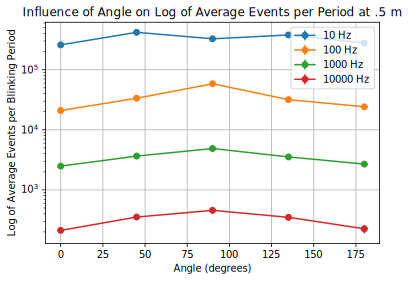
\includegraphics[width=0.475\textwidth]{../docs/fig/plots/angle/angle1.pdf}
			  \label{fig:angle_1}
			}
			% \subfloat[Influence of rotation of the UAV on the log of average number of events at 1 m.] {
			%   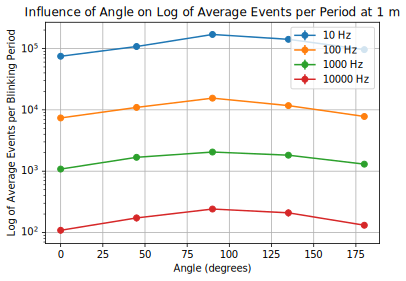
\includegraphics[width=0.5\textwidth]{./fig/plots/angle/angle2.pdf}
			%   \label{fig:angle_2}
			% }
			\subfloat[Influence of rotation of the UAV on the log of average number of events at 2 m.] {
			  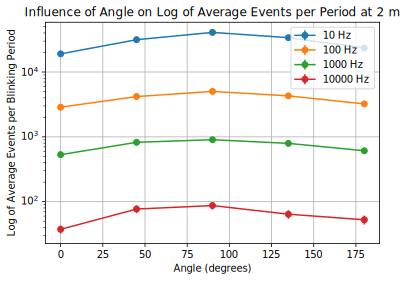
\includegraphics[width=0.475\textwidth]{../docs/fig/plots/angle/angle3.pdf}
			  \label{fig:angle_3}
			}
			\caption{
		  The influence of rotation angle on the log of average number of events at 0.5 m on \reffig{fig:angle_1} and at 2 m on \reffig{fig:angle_3}.
		  The distribution approaches the theoretical model with the increase of distance.
		  }
			\label{fig:angles}
		\end{figure}
	\end{frame}

	\begin{frame}{Light diffraction}
		%compare two leds from two different distances

		\begin{figure}
			\centering
			\subfloat[LED blinking at 10 Hz at 1.0 m] {
			  \includegraphics[width=0.5\textwidth]{../docs/fig/photos/led_10hz.png}
			  \label{fig:stars_1}
			}
			\subfloat[LED blinking at 1 kHz at 1.0 m] {
			  \includegraphics[width=0.5\textwidth]{../docs/fig/photos/led_1000hz.png}
			  \label{fig:stars_2}
			}
			\caption{
		  Two same LED light sources at 1.0 meters, blinking at 10 Hz and 1 kHz.
		  \reffig{fig:stars_1} shows a visible diffraction star (while being much brighter), while
		  \reffig{fig:stars_2} shows a
		  much more cicular source of light that is not as bright. \cite{lendermann2018computational}
		  }
			\label{fig:stars}
		\end{figure}
	\end{frame}

	\begin{frame}{RSSR}
		%mention the RSSR method

		These results will be used in the subsequent bachelor thesis, which will utilize the RSSR \cite{jung2014rssr}
		method, which measures the ratio of received light LEDs from multiple light sources.

		\begin{figure}
			\centering
			
			\subfloat[UAV with each LED blinking at a different frequency.] {
			  \includegraphics[width=0.45\textwidth]{../docs/fig/photos/rssr.png}
			  \label{fig:rssr1}
			}
			\hfill
			\subfloat[Calibration lattice.] {
			  \includegraphics[width=0.45\textwidth]{../docs/fig/photos/calibration.png}
			  \label{fig:calibration}
			}
			
		\end{figure}

	\end{frame}

	\begin{frame}[shrink=20]
		\frametitle{References}
		%\nocite{*}
		\begingroup
		\tiny
		\printbibliography[heading=none]
		\endgroup

		The source code can be found at:
		
		\url{https://github.com/kubakubakuba/mrs-uvdar-distance-estimator}.
	\end{frame}

\end{document}